% \addbibresource{../source/TASverif.bib}

% ****************************************
% *************************** Introduction
% ****************************************

\section{Introduction}\label{sec:intro}

Autonomous systems are systems that involve software applications, machines and people, which are capable of taking actions with no or little human supervision~\cite{Murukannaiah2020}.
%
Autonomous systems (AS) are pervasive in current society and set to become even more so with current technological growth trends and adoption rates. Systems with embedded artificial intelligence (AI) and machine learning (ML) algorithms can be found in numerous applications from mobile phones~\cite{mediumaiphones}, insurance pricing~\cite{kuo2020towards}, vacuum cleaners~\cite{tf_vacuum} and self-driving vehicles to medical diagnostics~\cite{kononenko2001machine}, detecting structural damage to buildings~\cite{avci2021review} and predicting the shape of protein molecules~\cite{alpha_fold} to name a few.
%
For successful adoption of, and reliance upon AS there needs to be demonstrable assurance of their trustworthy operation which becomes increasingly difficult for complex systems and changing environments.  
%
There is also growing use of machine learning in a range of safety-critical systems (SCSs), for example in the aerospace and automotive industry where low reliability of these systems could result in catastrophic failure and potentially loss of life or damage to property and the environment. These safety-critical autonomous systems present a complex but essential challenge to the safety assurance and verification community. 

Verification and validation (V\&V) is the process to gain confidence in the correctness of a system relative to its requirements. Prior to, and separate from verification, a specification must clearly define the trustworthy operational behaviour of the system and many challenges are associated with this task for autonomous systems~\cite{Abeywickrama2022}. 
%
% Conventional V\&V is principally concerned with assessing the system against a set of requirements, providing guarantees of functionality and assurance of safety.
%
If autonomous systems are to be fully accepted into society, there must be acknowledgement of, and evidence to show, compliance with a broad range of \emph{trustworthiness qualities}. 
%
A trustworthiness quality is defined here as a non-functional system property that enables adoption or promotes reliance in that system with \emph{trust stakeholders}. A trust stakeholder is a collection of entities or bodies that have a vested interest in the reliable operation of the system or otherwise seek assurance specific system properties. 
% 
A major challenge in verifying this broad category of trustworthiness qualities, are the lack of standards and regulations against which they can be evaluated. And whereas verification methods of assessing, for example, functional correctness are relatively mature, there also exists the challenge of developing robust assessment methodologies and metrics for these more nuanced trustworthiness qualities. 
%
% [maybe cut] For example, there are well defined rules for driving conduct and expected behaviour [UKHC] which could be verified using simulation based verification [harper22] but standards for social interaction, aesthetics or ethical behaviour are either non-existent or just emerging [EU directive for AI ethics]. 
%
This paper focuses on reviewing what trustworthiness means in the fields of AS, robotics, HRI and Cyber-Physical Systems (CPS) and how the application, criticality and level of autonomy influence trust priorities. 
%
We are aware of other factors contributing to trust, such as the broader epistemological or sociotechnical aspects of trust but will not consider these here, nor the process of gaining, maintaining or preventing the erosion of trust, e.g. see~\cite{Chiou2021}. We focus on technical aspects of trustworthiness relating to the system and outline the challenges associated with practical application of a presented assessment process. 

% ****************************************
% ***** V&V for AS in complex environments
% ****************************************

\subsection{V\&V for AS in complex environments} \label{sec:intro-vav}

A widely held tenet is that there can never be a suitable amount of verification that gives complete assurance for complex, safety-critical autonomous systems, although limits on reliability rates have been proposed~\cite{Butler1993}. Corroborative V\&V~\cite{webster2020corroborative} attempts to improve confidence through combining mutually consistent evidence from multiple and diverse assessment methods, e.g. formal, testing. 
%
But even this may not be enough for the diverse operational domains of some AS, e.g. automated vehicles in high-density urban areas, and thinking should move beyond verification at only the system design stage, to a more continuous operational evaluation such as runtime verification. Runtime verification brings other currently unresolved issues, such suitable oracle design~\cite{Leucker2009}, but some authors propose valid ideas to this using edge computing and cloud-based verification~\cite{CyRes20,eder2021cyres}. 
%
The use of \emph{serious games} can be another interesting opportunity for building trustworthiness in complex autonomous systems and has been used in the context of mission planning for NASA~\cite{Allen2018} and in a self-driving vehicle controller leveraging the power of crowdsourcing for test generation [ref test gen game, need to make github page, add code and youtube videos]. 

Further to this issue, are the lack of \emph{standards} against which some trustworthy qualities should be appraised and the \emph{methods} by which they should be evaluated. For example, there are standards for correct road driving conduct~\cite{highwayCode} but no ethical standards by which those driving decisions should be made [ref like trolley problem?]. 
%
Although headway is being made into developing standards for non-functional properties, such as guidelines for ethical AI [ref EU AI high level expert group], checklists for HRI best practice ~\cite{kraus2022trustworthy} and transparency~\cite{winfield2021ieee}, there are still areas that need attention, such as standards for adaptability, cooperation and fairness~\cite{Abeywickrama2022}. 
%
Where standards are lacking or immature will require engagement with \emph{trust stakeholders}, expert steering groups that can define and prioritise the necessary trustworthiness qualities for each subject domain or application. 

Additionally, there is more that can be done at the design stage to improve \emph{verifiability} [add ref]. Evidence for functional correctness is essential, but this must be supported with decision explanation~\cite{koopman2018toward} whilst maintaining intellectual property rights around, for example, sensitive software algorithms and trade secrets [ref]. 

In addition to assessing the AS trustworthiness, there must also be consideration to gain, calibrate and maintain user trust in the system~\cite{kok2020trust, Chiou2021}, as miscalibration of trust between system and user can have serious consequences~\cite{kok2020trust}. 


%\subsection{Document Structure}
% In the following, related work is reviewed in Section


% ****************************************
% ************** Trustworthiness Qualities
% ****************************************

\section{Trustworthiness of AS Qualities (TASQ)}\label{sec:tasq}

As computing and automation has developed, systems are now both more capable and users more reliant on them. This extension of capability has resulted in a broadening of the terms which encompass trustworthiness, as, for example, the important trustworthiness qualities of a calculator may be less numerous than those of a medical decision support system. Advancement in automation then, has led us to question and challenge these new capabilities, or, as some commentary has noted: with more automation comes more responsibility~\cite{Yazdanpanah2021}. 

Trust can be expressed in a number of ways and directions; trust the user has in the system, the objective trustworthiness of the system and the context in which the interaction between the two takes place~\cite{Hancock2021}. 
%
Trustworthiness can also been described as a the probability that a system holds some established property or quality, and that greater trustworthiness begets greater likelihood that the system may exhibit that quality. 
%
In this research we consider the trustworthiness of the system and the specific qualities that must be demonstrated, but we acknowledge the importance of the other mechanisms where human-system trust can be gained or lost in which there has been much contribution from the HRI, psychology and human factors community~\cite{Floridi2019,Lee2004,kok2020trust,Chiou2021,Kohn2021,kraus2022trustworthy}. 
%
Trustworthiness of autonomous systems in the context of this work then, results from objective assessment of the system with respect to a set of appropriate standards. 
%
There has been much academic deliberation on the specific qualities that comprise trustworthiness of AS, specifically for AI~\cite{Thiebes2021,Wing2021} and HRI~\cite{kraus2022trustworthy,atkinson2012trust}
%
Devitt argues that reliability and accuracy are the two central pillars of trustworthiness of AS and that all other properties stem from these, for example, stating that adaptability and redundancy are higher-order properties of reliability~\cite{devitt2018trustworthiness}. 

\cite{ts_foundation} state 5 facets of trustworthy software: Safety: The ability of the software to operate without causing harm to anything or anyone.Reliability: The ability of the software to operate correctly. Availability: The ability of the software to operate when required.
Resilience: The ability of the software to recover from errors quickly and completely. Security: The ability of the software to remain protected against the hazards posed by malware, hackers or accidental misuse.


% ****************************************
% ************************ Ontology of AS
% ****************************************

\subsection{Ontology of AS Trustworthiness Qualities}\label{sec:tasq-ont}

A trust ontology can be a useful definition to identify an independent set of important quality characteristics, where one category is not necessary influenced or related to its neighbours. These categories can be used to support clarity of communication and understanding of issues pertaining to, and of judgement in the assessment of, trustworthiness of autonomous systems. 

Lee \& Moray propose the categories for trust in automation: performance (consistent and stable behaviour), process (qualities or characteristics that govern behaviour), purpose (underlying motive or intent) and foundation (fundamental assumptions of natural and social order). These categories broadly capture the full gamut of trustworthy qualities but may be too broad and abstract for practical assessment purposes. 

Avizienis et al. proposes that a set of general concepts are required for dependable and secure computing, which may cover a wide range of applications and system failures, comprising; availability (readiness for correct service), reliability (continuity of correct service), safety (absence of catastrophic consequences on the user and the environment), integrity (absence of improper system alterations) and maintainability (ability to undergo modifications and repairs)~\cite{avizienis2004basic}. The focus here is on functionality and usability, but these categories may be too specific to computing and neglect verifiability and ethical considerations around AI.

Thiebes et al. argue for five foundational principles of trustworthy AS: beneficence (doing good), non-maleficence (not harming), autonomy (preserving human decision making), justice (fair and reasonable), and explicability (easily understood)~\cite{Thiebes2021}. These are based on and related to numerous other discussion on ethically principled foundations of trustworthiness and there is evidence of strong international collaboration and motivation in this area~\cite{Floridi2018,jobin2019global}. Whilst these categories are very important and capture ethical and regulatory considerations, they fail to capture the aspects of functionality and dependability of other voices in the community.

Cho et al. propose a STRAM ontology for measuring the trustworthiness of computer systems, based around four sub-metrics of: security (availability, confidentiality, integrity), trust (predictability, safety, reliability), resilience (adaptability, fault-tolerance, recoverability) and agility (efficiency, usability, timeliness), although again functional aspects are missing with the main focus being on security.

\begin{figure*}[]
    \centering
    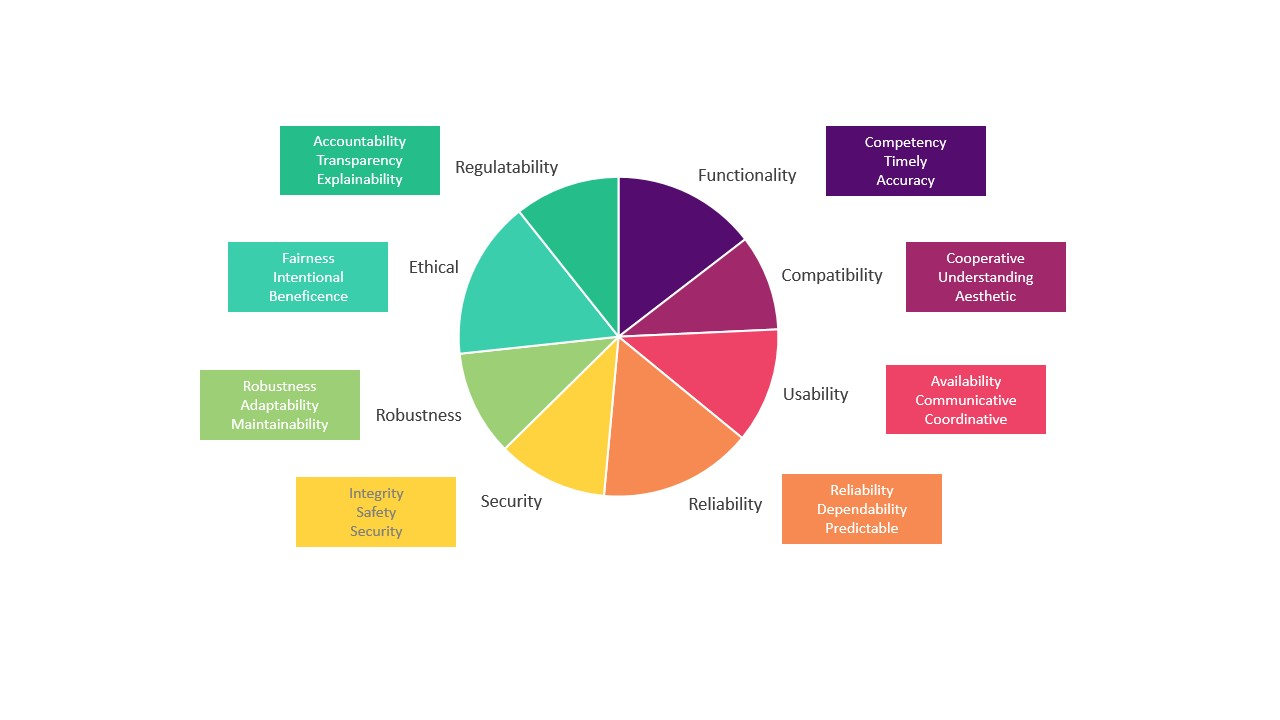
\includegraphics[width=0.98\linewidth, trim=2cm 4.5cm 2.5cm 2.5cm, clip]{\pathToOtherFiles/figures/trust_spectrum.jpg}
    \caption{Analysis of trust quality terms in the literature placed into categories, breakout box shows most cited words from each category.}
    \label{fig:trust_spectrum}
\end{figure*}

% ****************************************
% ********************* Existing Standards
% ****************************************

%----------------------------------------------------------------------------------Contributed by Dhaminda (Start)------------------------------------------------------------------------------------
%------------------------------------------------------------------------------------------------------------------------------------------------------------------------------------------------------------------------
\subsection{Standards for Autonomous Systems and Trustworthiness Properties}
% Contributed by: Dhaminda Abeywickrama
% 2 September 2022
% Autonomous systems are systems that involve software applications, machines and people, which are capable of taking actions with no or little human supervision~\cite{Murukannaiah2020}. %moved up to intro
The functionality of an autonomous system (i.e. what it is meant to do, what it does, and what it could do) evolves or changes over time. 
One of the main issues of adopting current standards and regulations with autonomous systems is the lack of consideration to the notions of \textit{uncertainty} and \textit{autonomy} \cite{Fisher2020}. 
Most conventional processes for defining system requirements assume that these are fixed and can be defined in a complete and precise manner before the system goes into operation \cite{Abeywickrama2022}. 
Also, in existing standards and regulations, the notion of autonomy is not their most characterizing feature where they are neither driven nor strongly influenced by it \cite{Fisher2020}. 
Most existing standards are either implicitly or explicitly based on the V\&V model, which moves from requirements through design onto implementation and testing before deployment~\cite{Jia2021}. 
However, this model is unlikely to be suitable for systems with the ability to adapt their functionality in operation; e.g.\ through interaction with other agents and the environment (e.g. as is the case with swarms); or through experience-driven adaptation as is the case with machine learning \cite{Abeywickrama2022}. 
%
\textcolor{red}{we have not yet mentioned systems with evolving functionality, this can be put in the introduction}
%
Autonomous systems with evolving functionality follow a different, much more iterative life-cycle. 
Thus, there is a need for new standards and assurance processes that extend beyond design time and allow continuous certification at runtime~\cite{Rushby2008}. 
In this context, lately, there have been several standards and guidance introduced by several industry committees and research groups. 
Now we provide an overview of several key efforts with any trustworthiness properties or ontologies supported by them.

In 2016, the British Standards Institution introduced the \textit{BS 8611} standard that provides a guide to the ethical design and application of robots and robotic systems \cite{BS8611}. 
Then, IEEE through its initiative Global Initiative on Ethics of Autonomous and Intelligent Systems initiated the development of a series of standards to address autonomy, ethical issues, transparency, data privacy and trustworthiness (IEEE P70XX, for e.g. IEEE P7001, P7007, P7010). 
\textit{IEEE P7001} standard describes measurable, testable levels of transparency for autonomous systems so that they can be objectively assessed and levels of compliance determined\cite{IEEE-P7001}. 
This standard outlines five stakeholder groups, and for each group it explains the structure of the normative definitions of levels of transparency. 
\textit{IEEE P7001} can be applied to assess the transparency of an existing system using a process of System Transparency Assessment, or to specify transparency requirements for a system prior to its implementation using a System Transparency Specification.
Meanwhile, the goal of \textit{IEEE P7007} standard is to assist in the ethically-driven methodologies for the design of robots and automation systems \cite{IEEE-P7007}.
For this, it provides a set of ontologies with different abstraction levels of concepts, definitions, axioms and use cases. 
IEEE P7001 mentions about a transparency concern, which is a property representing an explanation topic (e.g. fairness, safety, legality, reliability, accountability, responsibility, predictability, comprehensibility, justifiability, viability, coordination) describing the reason for explanations of agent behaviours. 
\textit{IEEE P7010} standard is used to measure the impact of AI or autonomous and intelligent systems on humans \cite{IEEE-P7010}. 

There are several standards and guidance related to machine learning in aeronautics, automotive, railway and industrial domains, e.g. AMLAS, EASA concept paper, DEEL white paper, AVSI report, LNE certification and UL 4600 standard \cite{Kaakai2022}.

\textit{Assurance of Machine Learning for use in Autonomous Systems (AMLAS)} provides guidance on how to systematically integrate safety assurance into the development of the machine learning components based on offline supervised learning \cite{Hawkins2021}. 
%AMLAS provides an explicit and structured safety case that the system is safe to operate in its intended context of use. 
AMLAS contains six stages, and the assurance activities are performed in parallel to the development of machine learning component. 
The process is iterative by design and feedback is used to update previous stages. 
In AMLAS, the safety requirements are always based on performance and robustness of the machine learning model. 
In a related work to AMLAS \cite{Ashmore2021}, the authors identify several phases in a machine learning life cycle (data management, model learning, verification and deployment) with their associated data. From an assurance view point, they consider several key properties the models generated by learning should exhibit: performance, robustness, reusability and interpretability.% (see Table\ref{table:1}).

The \textit{concept paper} by the \textit{European Union Aviation Safety Agency (EASA)} provides its first usable guidance for level 1 (human assistance) safety-related machine learning applications \cite{EASA2021}. 
%It provides means of compliance for the certification of safety-critical systems which rely on machine learning-based algorithms for their operation. 
This guidance provides a roadmap to create a framework for AI trustworthiness (\cite{EASA2021}, pg. 8). The framework describes three techniques for analysing trustworthiness (safety, security and ethics-based), which are linked with the ethical guidelines developed by the EU commission (accountability, robustness, safety, oversight, privacy and data governance, non-discrimination and fairness, transparency, and societal and environmental well being). 

The \textit{DEpendable and Explainable Learning (DEEL) white paper} aims to identify challenges in the certification of systems using machine learning and to define a set of high-level properties for that purpose, such as auditability, data quality, explainability, maintainability, resilience, robustness, specifiability and verifiability (\cite{Mamalet2021}, pg. 22–23). 

The \textit{Aerospace Vehicle System Institute (AVSI) report} on machine learning summarises their findings on safety and certification aspects of emerging machine learning technologies that are applied to safety-critical aerospace systems \cite{AFE2020}. This report provides several recommendations with respect to robustness, safety assurance, runtime assurance and interpretability when using machine learning in safety-critical applications. 

The \textit{UL 4600 standard} guides a user through the development of safety cases for fully automated vehicles (i.e. vehicles with no driver or supervisor) \cite{UL4600}. It is more of a standard of care and not a procedure for certification of fully automated vehicles. The \textit{Laboratoire National de Métrologie et d'Essais (LNE) certification} \cite{LNE2021} is a quality assurance standard for machine learning processes. The aim is to provide guidance for an applicant when obtaining certifications for their design, development, evaluation and maintenance in operational conditions. 
%----------------------------------------------------------------------------------Contributed by Dhaminda (End)------------------------------------------------------------------------------------
%------------------------------------------------------------------------------------------------------------------------------------------------------------------------------------------------------------------------

\subsubsection{Ontologies within Existing Standards}\label{sec:tasq-ont-stds}

The international standard ISO/IEC/IEEE 29119 describes software and systems engineering and part-4 covers software testing techniques and outlines 8 areas that testing should focus around: Functional Stability, Performance Efficiency, Compatibility
Usability, Reliability, Security, Maintainability, Portability~\cite{ISO29119}. 
%
This standard is primarily focused on software testing and so some of these categories, although useful, includes jargon specific to computing systems which were not repeated in any other literature pertaining to AS more generally and therefore less user-friendly. However, part-13 of ISO29119 sets out standards specifically for testing AI-based software systems which extends these quality characteristics to include AI-specific qualities such as: flexibility (range of behaviours), adaptability (ease of modification or achieving flexibility), autonomy (unsupervised ability and level of control), evolution (behaviour adaptation over time), bias (e.g. due to discrimination, historic bias, uneven sampling), transparency (access to data and algorithms and decision interpretability) and determinism (same output for given input) as well as consideration to ethical specifications and side-effects such as reward hacking. 

FUTURE:ISO standard on "quality model for AI-based systems"


DIN SPEC 92001 is a standard to help ensure quality in AI systems. Part 2 of the standard (92001-2) describes three pillars responsible for AI quality, namely: functionality and performance, robustness and comprehensibility - look into

% maybe drop
The NIST Framework for Cyber-Physical Systems [ref] details a list of trustworthy `aspects' and `concerns' in addition to operational and business concerns for CPS and also includes some excellent case studies to show a complete end-to-end analysis, whilst Balduccini goes on to draw reasoning about the trustworthy properties set out in the framework in a UML/XML language [ref].  
%



% notes:

% Existing standards on verification (from Rudas 2020): P1872.1, P2817, P7000 and P7007.

% Safety of autonomous systems (from Hawkins 2022): UL4000 [Underwriters Laboratories. Standard for evaluation of autonomous products, 2020] or SCSC-153B [Safety of Autonomous SystemsWorking Group. Safety assurance objectives for autonomous systems, 2022. URL: https://scsc.uk/scsc-153B]


% Ethical framework for AI~\cite{Floridi2018} ``offer 20 concrete recommendations to assess, to develop, to incentivise, and to support good AI"

% Porter2022 presents an ethical assurance argument for AS, extending the assurance case considered for safety to include ethical standards

% devitt2018trustworthiness 

% What human factors are considered eg. ISO29119

%\textcolor{red}{Dhaminda to contribute here?}


A spectrum of qualities is presented that captures the broad definition of trustworthiness of AS from the literature, see Table~\ref{tab:quals}. A full list of the quality terms reviewed can be found at~\cite{tsl_git}.

\begin{table*}[t]
\caption{Trustworthiness qualities ontology}\label{tab:quals}
\centering
\begin{tabular}{ll}
\toprule
Trustworthiness  & Definition                \\ 
Quality Category   &   \\ \midrule

Functionality & Ability of a system to not enter a failure mode, to be able to execute tasks required of it without \\
&fault, to achieve a goal state (liveness), and do so within permitted use of resources.\\

Compatibility & Degree to which the system can exchange information with users or other systems, be transferred to\\
&other environments and the ability to share the same environment with other autonomous agents.\\

Usability & Extent to which the system is available and responsive and can be used to achieve specified goals\\
&with effectiveness, and satisfaction in a specified context.\\

Reliability & Degree to which the system performs specified functions under specified conditions for a specified\\
&period of time in a consistent manner.\\

Security & Protection against intentional subversion or forced failure, malicious access, use, modification, \\
&destruction, or disclosure. Defining, achieving, and maintaining confidentiality, integrity, availability, \\
&non‐repudiation, accountability, authenticity, and reliability of the system. \\

Robustness & Ease with which the system can overcome adverse conditions and be maintained or modified to change\\
&or add capabilities or to operate at new scales, correct faults or defects, improve performance or other\\
&attributes and to adapt to new environments.\\

Ethical & Ability to demonstrate beneficence and non-maleficence, fair and reasonable behaviour, to preserve\\
&human decision making and be easily understood\\

Regulatability & Ease in which the system is verifiable, readable, explainable, transparent and understandable in a \\
&manner to support regulation, appropriate trustworthy metrics and specifications.\\

\bottomrule
\end{tabular}

\label{tab:ontology}
\end{table*}


% ****************************************
% **************** Application Criticality
% ****************************************
\section{Application Criticality} \label{sec:appcrit}

What is not considered a great deal in the literature is application criticality; what application the AS is used for and if this should change the significance of specific trustworthiness qualities. Applications will need more emphasis on certain trustworthy qualities depending on where the system is most vulnerable to violating trust. 
%
\textcolor{red}{Arianna, is there a focus in ethics on where the power is held? and whom can be prejudiced/discriminated against?} 
%
For example, a self-driving vehicle, or indeed any safety critical system, must have emphasis on safety, possibly to the detriment of other qualities. 

DIN SPEC 92001-1 describes a \emph{quality meta model} and distinguishes between high risk systems that have safety, security, privacy and ethical relevance and those that do not (low risk), delineating applications into two risk classes~\cite{Englisch2019} which can be assessed using an appropriate risk assessment process, e.g. HAZOP, FMEA, SHARD. High risk applications must commit evidence of system trustworthiness based on these categories (or must be justified) whilst low risk systems are less strict.

Whilst this DIN SPEC approach is commendable, it does not go far enough to filter trust qualities based on the application and identify the key qualities required for assessment. The risk assessment process can be used to identify those qualities which are most pertinent to the application which can be prioritised, included or discarded entirely. For example, there may be an application with strong safety requirements but little to none regarding privacy. 

Fisher 2021 asks if there are some rules that are more important that others, are all rules born equal? Context and application, social and cultural norms will all influence this answer. An example may be the ease with which breaking the speeding limit is observed in driving behaviour, but other driving conduct rules are broken less often, such as driving through a red traffic signal light.

\subsection{Decision Making Complexity} \label{sec:appcrit-dec}

Within application criticality comes decision making complexity, the complexity of the process the AS must navigate in order to achieve the task goal. This could be considered in terms of the system and the constraints in the environment or action space to allow or prevent the system reaching a number of potential future states. A autonomous vacuum cleaner, for example, is physically constrained to a small 2-dimensional plane (area to be cleaned) and can successfully function with a small action space (stop, rotate, drive) where decisions are reactively made based on a few simple sensor inputs (avoid close object). 
%
Contrast this to, for example, any system that requires a perception stack to interpret dynamic physical scenes, such as a self-driving vehicle, which must identify and extrapolate objects and their future states (pedestrians), environmental conditions (road furniture, fog) and static or temporary rules that require interpreting (road signs, traffic cones) which will all contribute to a decision, which is also exacerbated by the potential harm that can result if a wrong decision is made. 
%
Decision making complexity needs to be considered when judging the risk level of the application, and the associated trust qualities should be elevated accordingly, where applications that have high risk associated with particular qualities, those qualities should be elevated to higher risk levels and be assessed accordingly (see Section~\ref{sec:AssFramVis}).  

\subsection{Potential harm (from failure)} \label{sec:app-harm}

Qualities that are principally connected to the functionality of the AS, are required for trustworthiness. A vacuum cleaner with poor coordination can do limited harm to users, but the same lacking quality in a robotic assistant, say, may fail to be accepted as trustworthy and also cause potential harm. Therefore, the trust quality must be elevated to a high risk level.
%
A risk assessment process should be able to identify such critical properties that can follow through the verification process. 


% ****************************************
% *********************** Automation Level
% ****************************************
\section{Automation Level} \label{sec:autlev}

The level of automation is an important consideration which relates to what qualities the system should present, our reliance and vulnerability to the system and hence the criticality of the application. A good description of automation levels are given by SAE International~\cite{SAEJ3016}. 
%
Fisher et al. describe \emph{automation scope} which, alongside the level of automation, describes the sophistication of potential system actions and the ability to achieve complex task goals~\cite{Fisher2021}. 
%
Alongside scope, agency (independent acting or decision making) and whether to be reactive (responding to a situation or stimulus) or proactive (creating a situation) in action decision are also factors to consider within automation level.
%
Greater scope, greater responsibility [ref]
%
% The example given is that two automated vacuum cleaners can both clean and avoid obstacles, but one schedules action to avoid human disruption. 
%
But automation scope is simply an aspect of non-functional AS qualities, of which compatibility, which includes co-existence and harmony, are aspects of automation that would naturally extend the scope of the system. 





% ****************************************
% ******************* Assessment Framework
% ****************************************
\section{Assessment Framework Vision} \label{sec:AssFramVis}

\begin{figure*}[]
    \centering
    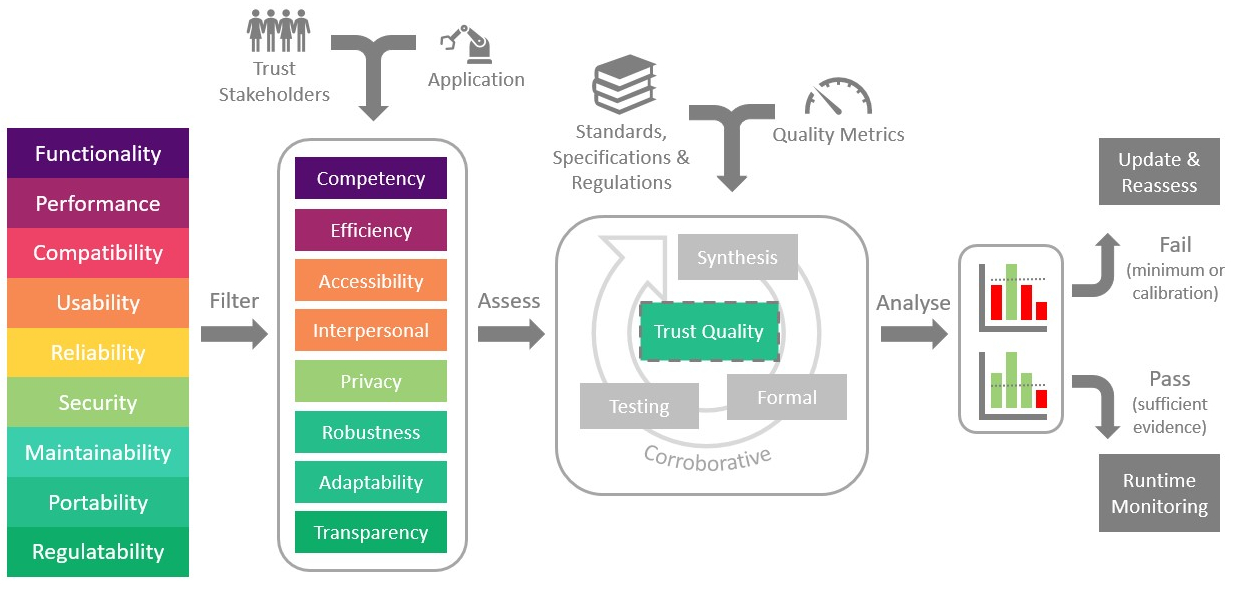
\includegraphics[width=0.98\linewidth, trim=0.3cm 1.0cm 0.5cm 0.5cm, clip]{\pathToOtherFiles/figures/tas_ver.jpg}
    \caption{AS trustworthiness assessment process}
    \label{fig:tas_ver}
\end{figure*}

Below is a checklist for assessment of AS trustworthiness:

\subsection{TASQ Categories}

After reviewing the literature, a comprehensive ontology has been derived based on TASQ. 

\subsection{Application Criticality Analysis}

Which TASQ to include in your application? Are all qualities relevant? How can quality relevance be objectively assessed? What inputs are required from trust stakeholders? How does automation level affect the choice?    

\subsection{TASQ Assessment with Corroborative V\&V}


Kress-Gazit et al. state that assessment in the correctness of AS can be broken down into four approaches: synthesis of correct-by-construction systems, formal verification at design time, runtime verification or monitoring, and test-based methods~\cite{kress2021formalizing}. 
%
This assessment uses all four approaches both at design time, during operation (runtime) and as a consequence of development iteration or update. 



\subsection{Standards and Regulations}

What standard for each quality? Is there a relation/pattern? Can we map standards to qualities or is it application based? 


\subsection{Metrics}
Floridi suggests the need for agreed upon metrics for trustworthiness of AI systems and suggests an  AI Trust comparison index, metrics are needed for benchmarking AI suitability to the public. 
%
Rudas and Haidegger also supports the idea of agreed upon metrics from the verification community that can be used to ensure reliability of complex autonomous systems~\cite{Rudas2020}. Wang et al. go further and propose a  theoretical framework of \emph{tripartite trustworthiness} covering; \emph{to-be trust} (trustfulness of an entity or structure), \emph{to-do trust} (trust in an action or behaviour) and \emph{system trust} (a statistical runtime evaluation of performance) and set out 18 formal definitions~\cite{Wang2020}. 
%
Garbuk presents the idea of \emph{applied intellimetry} to assess the quality of AI systems by formulating a list quality characteristics in a functional characteristic vector~\cite{garbuk2018intellimetry}. 
%
Kaur et al. suggest explainability metrics based on the euclidean distance between the system output compared to a panel of experts~\cite{kaur2021trustworthy}. 
%
trustworthiness of computer systems using metrics designed to assess security, trust, resilience and agility~\cite{cho2019stram}

Bolster and Marshall proposes the idea of \emph{multi-vector trust metrics} for networks of autonomous systems, indicating that the use of \emph{grey relational analysis}, a theory to describe and model uncertainty, could be beneficial for combining temporally sparse, low fidelity metrics with unknown statistical distributions~\cite{Bolster2014}. 

For data-centric and highly objective measures of trust, operators such as accuracy, precision and recall can be useful for functionality metrics. Questions over what is the ground truth is, a sample of the real world, artificially augmented, and if the data is ethically sourced are all additional factors to be considered. We may even be more abstract and use \emph{task completion} - this will confluence with other assessment areas.



\subsection{Analysis \& Visualising Trust}

Whereas metrics for the development and regulation community may be highly technical, those that are public facing must be presented in a user-friendly manner that will attain and hold trust in the user, whilst maintaining the meaning of salient information without clouding in jargon [ref]. 

As suggested by Floridi, public confidence in AI-based systems could be bolstered with an internationally recognised index for trustworthy AI, such as a \emph{trust comparison index} or AI \emph{star rating}. A vision of this rating is shown in Table XXX. Much like an internet browser may convince users of their safety on a web page through some means, e.g. icons, coloured indicators, a similar approach could be taken with AS applications be that through cyber or physical means.


Corroborative, mutually consistent evidence from diverse methodologies provides assurance that is greater in quality than evidence from single sources and is the only process that can result in the highest TASQ rating. Evidence that fails to corroborate, although does not fail in itself, may be considered equivalent to single-source evidence and therefore, although not a failure, can only provide evidence for low risk applications.


If the risk assessment analysis deems the quality not to be critical then the minimum threshold for the specific metric of that quality can be relaxed for a passing grade. 

\begin{table*}[t]
\caption{Trustworthiness Autonomous Systems Quality (TASQ) star rating comparison index}\label{tab:tasq_rating}
\centering
\begin{tabular}{lll}
\toprule
TASQ  &  Assessment & Application \\ 
Rating & Description & Class \\ \midrule

\FiveStar & Single assessment method, meets minimum compliance  & low risk applications only\\
&with standards for low risk applications & \\

\FiveStar\FiveStar & 1-2 assessment methods where appropriate, meets recommended & low-moderate risk applications\\
& compliance level and attempt to calibrate user trust & \\

\FiveStar\FiveStar\FiveStar & evidence from at least 2 diverse assessment methods,  & any risk level applications\\
&meets full compliance guidelines and extensive  &\\
&user trust calibration&\\

\bottomrule
\end{tabular}

\label{tab:tasq_rating}
\end{table*}



\subsection{Insufficient Trust: Update \& Reassessment}



\subsection{Sufficient Trust: Monitoring}











\subsection{Future Challenges in Standards} \label{sec:AssFramVis-fut}

Riaz et al.~\cite{Riaz2018} suggest the idea of using social norms and human emotions as a standard by which better self-driving controllers may be developed. This idea sets the way for not just development of higher functioning AS, but also standards of trustworthiness by which they can be judged. Although there is much scholarly work on the theory and modelling of social norms, e.g.~\cite{hechter2001social}, there is yet to be published a standard that could be used to objectively assess an autonomous system. 

In some cases, e.g. driving, legislation on appropriate conduct is presented to society in the form of guidelines such as the UKHC in the UK~\cite{highwayCode} but must be translated to a computer readable format to act as an appropriate standard, or set of assertions~\cite{harper2021safety}, if these guidelines can be used to assess AS trustworthiness. A similar process will have to be undertaken for other standards which have yet to be defined, e.g. cooperation, fairness or verifiability, to ensure all aspects of trustworthiness can be assessed. 


% ****************************************
% ********************* Existing Standards
% ****************************************

\subsection{Assessment Methods \& Corroborative Evidence} \label{sec:AssFramVis-AssMthds}
Gaining reliability assurance of SCASs using testing alone is unfeasible given the often high-dimensional operational state space. Multiple testing methodologies should be employed where appropriate, e.g. verification, falsification and testing, [Harper Corroborative 2022] combining mutually consistent evidence from multiple and diverse assessment methods will raise the confidence in system trustworthiness.

Knowledge of the internal state of the system is often hidden, e.g. blackbox, due to IP and commercial sensitivity, but whitebox access will be essential for certain aspects of trustworthiness assessment. This may not need to reveal sensitive algorithms but just enough information through observability points in the software architecture could go a long way to understanding if automated decisions are made for the right reason~\cite{koopman2018toward}. 



% ****************************************
% ********************* Existing Standards
% ****************************************

\section{Conclusion} \label{sec:conc}






% ***********************************
% ***********************************
% ***********************************
% notes

% %
% 

% \subsection{Swarm Trustworthiness Qualities \& Assessment}\label{sec:verification-qualities-swarm}
% Robustness, scalability and adaptability are considered as being particularly useful qualities of swarm trustworthiness, although this list could be extended to cover many other trustworthy qualities [https://github.com/TSL-UOB/TAS-Verif]. 
% %
% \subsubsection{Trust Quality: Robustness}
% Robustness is the degree to which the system can function correctly in the presence of invalid inputs or stressful conditions~\cite{ISO24765}. For a swarm application invalid or stressful inputs could be, for example, individual agents failing, poor environmental illumination or limited network connectivity. \textcolor{red}{JAMES - are there other robustness factors to consider here for swarms?}. 
% %
% A suitable verification task may be to find the limits of robustness either through simulation and/or physical trials of task success to ensure that this meets the specifications. 
% %
% A swarm system operating in a bound environment with a fixed number of allowable agent actions is a relatively constrained problem compared to, say, a self-driving vehicle. A swarm that chooses from a fixed set of actions (e.g. behaviour tree) is well suited to verification via formal modelling. 
% %



% \subsubsection{Trust Quality: Scalability}
% Scalability is defined as...How do autonomous systems (swarms) of increasing scales affect trust? \textcolor{red}{JAMES - my interpretation of scalability would be how well/easily can the system be operated at a larger size. Increasing the size could impact on other functional and non-functional requirements, e.g. box delivery rate, collision frequency, user acceptance. Are you intending to explore the knock-on/secondary effects or was there something specific to size you wanted to explore?}. Trustworthy scalability metrics could comprise performance analysis give a change in swarm scale, usability of the swarm given the larger size and safety properties concerning collisions (tbd with James). 

% \subsubsection{Trust Quality: Adaptability}
% Adaptability is the degree to which a system can effectively and efficiently be adapted for different or evolving hardware, software or other operational or usage environments~\cite{ISO24765}. For a swarm application, this could be operating well with environmental obstructions, e.g. blocked path in a warehouse and having to find another route. In this case effective trustworthy metrics could be based around agent idle times (time not spent doing something useful) and recovery rates (speed at which a new route is found) when the swarm encounters a blocked paths. Additionally application performance metrics could be used to assess adaptability of swarms, for example task success rates in a find-and-fetch operation could be used for the swarm in a new building layout.

% \subsubsection{Trustworthiness of Emergent Behaviour}
% \textcolor{red}{Do we need to say here about emergent behaviours that cannot be assessed at the agent level? Or are we steering clear?}
% %
% \subsection{Trustworthiness Assessment Methods}\label{sec:verification-qualities-methods}
% Different verification methods will be more or less suitable to different domains based on the application. 
% %
% Formal verification requires a model of the system written in a formal language and can be used to prove a system (e.g. swarm) property is consistent against an \emph{entire} parameter space. This is in contrast to \emph{sampling} the parameter space if using a testing method, e.g. simulation technique. Formal verification provides a proof of assurance against single properties but the model generation can be non-trivial and the technique is not always suitable for complex systems operating in unbound domains, i.e. high dimensional parameter space. 
% %
% However, a swarm system operating in a bound environment with a fixed number of allowable agent actions is a constrained problem relative to, say, a self-driving vehicle. A swarm of robot agents that use a fixed set of actions (e.g. behaviour tree) is exactly suited to verification via formal model. 
% %
% Formal methods have been demonstrated to show robustness of a swarm to network connectivity loss using probabilistic finite state machine (PFSM) verification~\cite{Winfield2008} and is a valid method for this application. 
% %
% Although formal models can give assurance against an entire range of parameters, a drawback is that only gives assurance of the \emph{model} and there may be distinct difference between the model and the real system. This is where \emph{testing} methods, such as simulation based verification, can fill the gap. 

% % Testing-based methods can be used in a complementary and even corroborative manner to support a formal analysis. Corroborative V\&V seeks to combine mutually consistent evidence from multiple and diverse assessment methods will raise the confidence in system trustworthiness~\cite{harperFMAS22}. Physical and Simulation-based verification methods execute a single test case where a single output will be monitored as a pass or fail, and multiple test cases are used to build a \emph{test suite}. Testing techniques therefore rely heavily on test generation to produce a diverse and challenging test suite, a set of stimulus that will complement any formal assessment but also test any model assumptions and the bounds of the operational domain (edge cases). 

% Many techniques can be employed to build a suitably diverse test suite~\cite{MarkUtting2012} including; random test generation, manually written test cases (based on historical evidence or accidentology), fault-based test selection, requirements coverage based and agent-based~\cite{chance2020agency}. 
% %
% There are also assertion-based techniques that can be used to prove that the system complies with a set of provided rules, e.g. diving conduct for self-driving vehicles~\cite{harper2021safety}. 

% Runtime verification techniques can also be utilised as a post-design strategy to trustworthiness assurance, where an oracle is used to compare current and expected behaviour~\cite{Leucker2009}. Runtime verification requires a suitable oracle to be defined which sets the expected bounds of operation, similar to a pattern-of-life model, and can be useful for complex systems where exhaustive design-time verification is intractable and if the system can be expected to change regularly, e.g. software updates pushed regularly without time for a complete system re-verification. 

% % ******************** TODO
% Verification of the trust qualities of robustness, scalability and adaptability for a swarm are suited to a mix of formal and testing-based verification. A PFSM approach could be suitable to prove system robustness to network connectivity and task completion rate~\cite{Winfield2008}. Complementary to this, simulation should be used for assertion-based analysis of the system relative to the requirements, to ensure the system behaves as specified. 
% %
% Additionally, simulation may be used for capturing scalability information by increasing the swarm size, and reliability information compiled from long horizon observations. 
% %
% Where long-horizon testing is not feasible but high reliability is needed for low probability faults, e.g. safety critical aspects of the system, then reliability models can be used to estimate future fault rates that can be assessed against a specified \emph{fault tolerance level}~\cite{Butler1993}. 
% % Arguments of high reliability often assume that isolated components fail independently which is a parallel that can be drawn to a swarm of individual robot agents. 
% %
% Physical testing should be done to validate formal and simulation-based methods and potentially explore scenarios not possible in either of the non-physical methods. As physical testing is usually the more costly method, a test plan should set out and prioritise the most important trust qualities to analyse, e.g. safety-critical testing may be a priority. Validation of simulated results will help to build a strong and corroborative argument of swarm trustworthiness.